\documentclass[11pt]{article}
\usepackage{times}
\usepackage{geometry}
\geometry{margin=0.5in}
\usepackage{graphicx}

\vspace{-50pt}
\title{EE577B HW2 -- Part B Explanation}
\author{}
\date{}

\begin{document}
\maketitle

\vspace{-50pt}

\section*{Explanation of Delay Models}

The five OR gate models exhibit different behaviors due to the type of delay and assignment used in Verilog. The simulation results can be understood as follows:

\begin{itemize}
    \item \textbf{At time 0 ps:} All outputs are unknown (x) because no assignment has occurred yet. The processes only schedule updates after the first input change. The continuous assignment with delay also does not resolve immediately.

    \item \textbf{At time 4000 ps:} Inputs changed at 0 ps and all models update after 4 ns. Since $(A | B) = 1$, all outputs are equal to 1.

    \item \textbf{At time 7000 ps:} Inputs changed at 7 ns but the 4 ns delay has not yet expired. Therefore, all outputs remain at 1.

    \item \textbf{At time 11000 ps:} The effect of the 7 ns input change is visible. The inter-statement inertial models (\texttt{or\_block\_inter}, \texttt{or\_nba\_inter}) still show 1 because the short 0 pulse was filtered out. The intra-assignment transport models (\texttt{or\_block\_intra}, \texttt{or\_nba\_intra}) update to 0 since they propagate every input event after the programmed delay. The continuous assignment with delay (\texttt{or\_continuous}) also updates to 0, consistent with inertial delay behavior.

    \item \textbf{At time 14000 ps:} Inputs change again but the outputs have not yet been updated because the 4 ns delay has not elapsed. The values remain the same as at 11000 ps.

    \item \textbf{At time 15000 ps:} The non-blocking intra-assignment model (\texttt{or\_nba\_intra}) shows a temporary 1. This is because the input value of 1 at 11 ns was scheduled to appear at 15 ns, reflecting the transport nature of intra-assignment delays. The other models do not show this change.

    \item \textbf{At time 18000 ps:} The effect of the input change at 14 ns is visible. All models update to 0, with the inertial models showing the stable 0 after the full delay and the transport models having also settled to 0.
\end{itemize}

\section*{Waveforms}

        \begin{figure}[h!]
            \centering 
            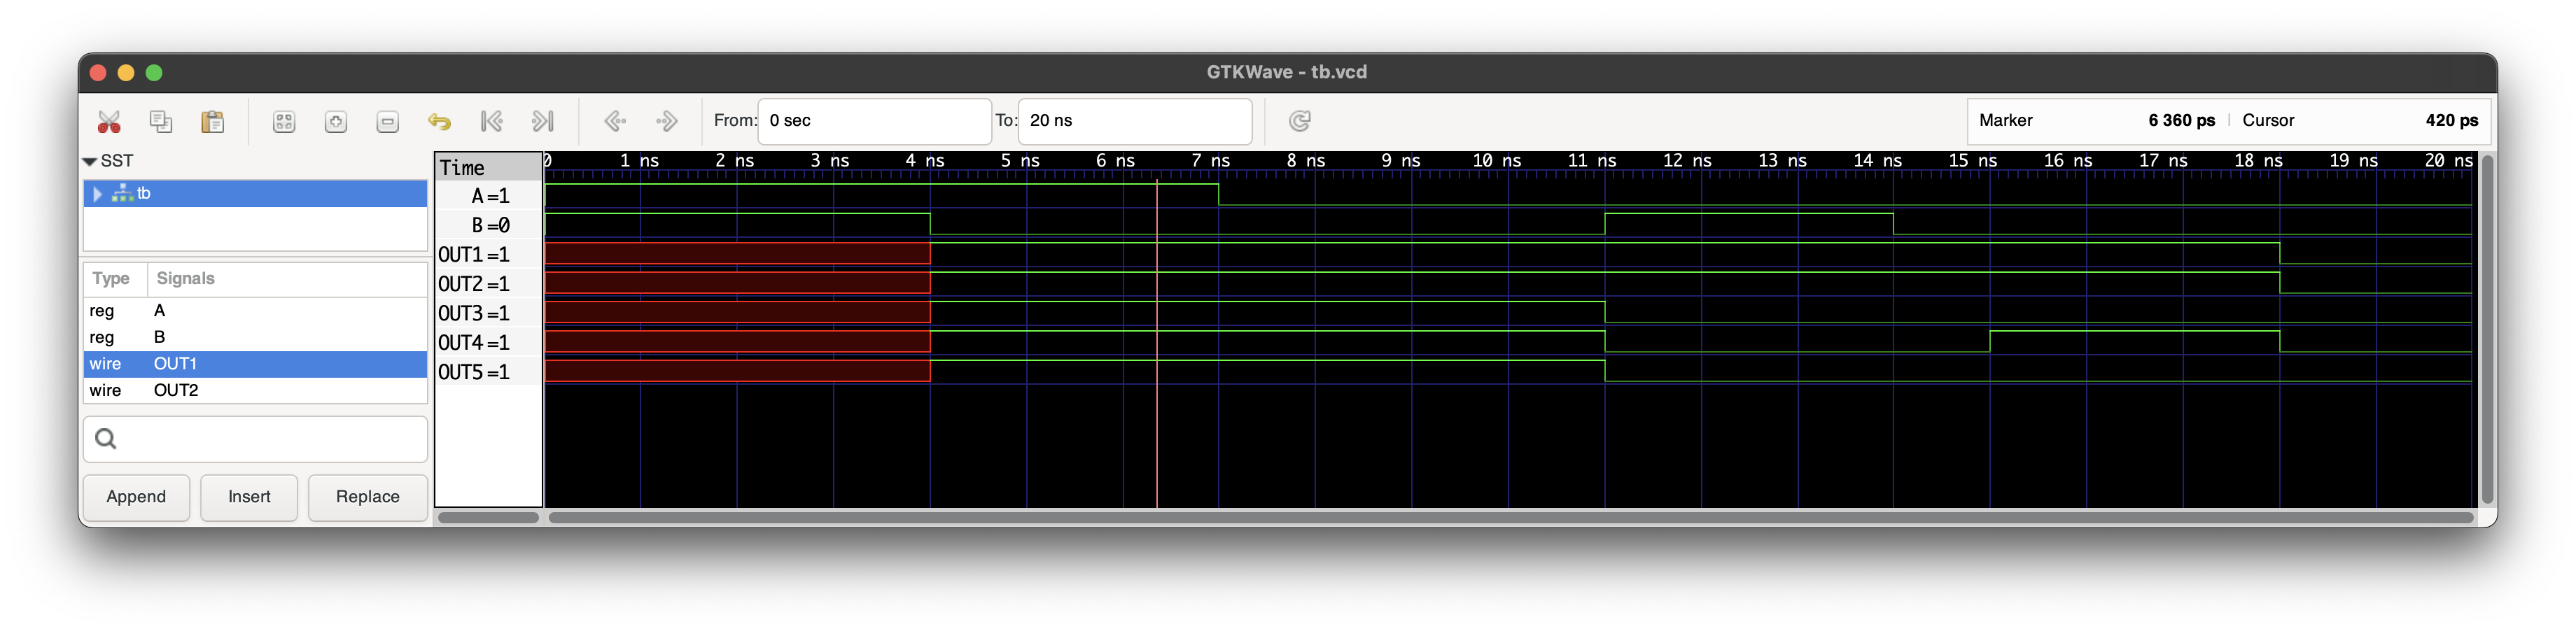
\includegraphics[width=0.7\textwidth]{B_delay.png}
        \end{figure}


\section*{Summary}
Inertial delays (inter-statement assignments and continuous assignments) filter out short pulses, while transport delays (intra-assignment assignments) propagate every event after the delay. Blocking versus non-blocking determines when in the simulation cycle the updates are applied, which explains the subtle differences in timing between the models.


\end{document}

